\chapter{Stack}
Typical scenarios to use stack:
\begin{itemize}
	\item {\color{blue}{Bracket matching}} in {\color{blue}{expression evaluation}}.
	\item Transforming {\color{blue}{recursive methods}} to {\color{blue}{iterative methods}} (because the {\color{blue}{call stack}} is involved in recursive methods.)
\end{itemize}

\section{LC 1047 - Remove All Adjacent Duplicates In String}
You are given a string {\colorbox{CodeBackground}{\lstinline|s|}} consisting of lowercase English letters. \\

A \ul{duplicate removal} consists of choosing two adjacent and equal letters and removing them.\\

We repeatedly make \ul{duplicate removals} on s until we no longer can.\\

Return the final string after all such duplicate removals have been made. (It can be proven that the answer is unique.) \\

Examples:
\begin{itemize}
\item {\colorbox{CodeBackground}{\lstinline|s = "abbaca" --> "ca"|}}
\item {\colorbox{CodeBackground}{\lstinline|s = "azxxzy" --> "ay"|}}
\end{itemize}

\subsection*{Solution - Stack}
\begin{lstlisting}
std::string removeDuplicates(std::string s) {
  std::stack<char> stk;
  for (char c : s) {
    if (!stk.empty() && stk.top() == c) {
      stk.pop();
    } else {
      stk.push(c);
    }
  }
  std::string result;
  while (!stk.empty()) {
    result += stk.top();
    stk.pop();
  }
  std::reverse(result.begin(), result.end());
  return result;
}
\end{lstlisting}

\section{LC 0020 - Valid Parentheses}
Given a string s containing just the characters {\colorbox{CodeBackground}{\lstinline|'('|}}, {\colorbox{CodeBackground}{\lstinline|')'|}}, {\colorbox{CodeBackground}{\lstinline|'\{'|}}, {\colorbox{CodeBackground}{\lstinline|'\}'|}}, {\colorbox{CodeBackground}{\lstinline|'['|}} and {\colorbox{CodeBackground}{\lstinline|']'|}}, determine if the input string is valid.\\

An input string is valid if:
\begin{enumerate}
	\item Open brackets must be closed by the same type of brackets.
	\item Open brackets must be closed in the correct order.
	\item Every close bracket has a corresponding open bracket of the same type.
\end{enumerate}

\subsection*{Solution}
\begin{lstlisting}
bool isValid(std::string s) {
  std::stack<char> stk;
  for (char c : s) {
    switch (c) {
      case '(':
      case '{':
      case '[': stk.push(c); break;
      case ')':
        if (!stk.empty() && stk.top() == '(') {
          stk.pop();
          break;
        } else {
          return false;
        }
      case '}':
        if (!stk.empty() && stk.top() == '{') {
          stk.pop();
          break;
        } else {
          return false;
        }
      case ']':
        if (!stk.empty() && stk.top() == '[') {
          stk.pop();
          break;
        } else {
          return false;
        }
    }
  }
  return stk.empty();
}
\end{lstlisting}

\section{LC 0032 - Longest Valid Parentheses}

\section{LC 1249 - Minimum Remove to Make Valid Parentheses}
Given a string s of {\colorbox{CodeBackground}{\lstinline|'('|}} , {\colorbox{CodeBackground}{\lstinline|')'|}} and \ul{lowercase} English characters.\\

Your task is to remove the minimum number of parentheses, i.e., {\colorbox{CodeBackground}{\lstinline|'('|}} or {\colorbox{CodeBackground}{\lstinline|')'|}}, so that the resulting \ul{parentheses string} is valid and return the valid \ul{parentheses string}. \\

Formally, a \ul{parentheses string} is valid if and only if:
\begin{itemize}
\item It is the empty string, contains only lowercase characters, or
\item It can be written as {\colorbox{CodeBackground}{\lstinline|AB|}} ({\colorbox{CodeBackground}{\lstinline|A|}} concatenated with {\colorbox{CodeBackground}{\lstinline|B|}}), where {\colorbox{CodeBackground}{\lstinline|A|}} and {\colorbox{CodeBackground}{\lstinline|B|}} are valid  strings, or
\item It can be written as ({\colorbox{CodeBackground}{\lstinline|A|}}), where {\colorbox{CodeBackground}{\lstinline|A|}} is a valid string.
\end{itemize}

Examples:
\begin{itemize}
\item {\colorbox{CodeBackground}{\lstinline|s = "lee(t(c)o)de)" --> "lee(t(c)o)de" or "lee(t(co)de)" or "lee(t(c)ode)"|}}
\item {\colorbox{CodeBackground}{\lstinline|s = "a)b(c)d" --> "ab(c)d"|}}
\item {\colorbox{CodeBackground}{\lstinline|s = "))((" --> ""|}}
\end{itemize}

\section{LC 0084 - Largest Rectangle in Histogram}

\section{LC 0150 - Evaluate Reverse Polish Notation}
You are given an array of strings {\colorbox{CodeBackground}{\lstinline|tokens|}} that represents an arithmetic expression in a \href{https://en.wikipedia.org/wiki/Reverse_Polish_notation}{Reverse Polish Notation}.\\



Evaluate the expression. Return an integer that represents the value of the expression.\\

Note that:
\begin{itemize}
	\item The valid operators are {\colorbox{CodeBackground}{\lstinline|+|}}, {\colorbox{CodeBackground}{\lstinline|-|}}, {\colorbox{CodeBackground}{\lstinline|*|}}, and {\colorbox{CodeBackground}{\lstinline|/|}}.
	\item Each operand may be an integer or another expression.
	\item The division between two integers always truncates toward zero.
	\item There will not be any division by zero.
	\item The input represents a valid arithmetic expression in a reverse polish notation.
	\item The answer and all the intermediate calculations can be represented in a 32-bit integer.
\end{itemize}

Examples:\\
{\colorbox{CodeBackground}{\lstinline|["2", "1", "+", "3", "*"] -> ((2 + 1) * 3) -> 9|}}\\
{\colorbox{CodeBackground}{\lstinline|["4", "13", "5", "/", "+"] -> (4 + (13 / 5)) -> 6|}}

\section{LC 0224 - Basic Calculator I}
Given a string {\colorbox{CodeBackground}{\lstinline|s|}} representing a valid expression, implement a basic calculator to evaluate it, and return the result of the evaluation.
\begin{itemize}
	\item {\colorbox{CodeBackground}{\lstinline|s|}} represents a valid expression, consisting of digits: {\colorbox{CodeBackground}{\lstinline|+|}}, {\colorbox{CodeBackground}{\lstinline|-|}}, {\colorbox{CodeBackground}{\lstinline|(|}}, {\colorbox{CodeBackground}{\lstinline|)|}}, and {\colorbox{CodeBackground}{\lstinline|' '|}}.
	\item {\colorbox{CodeBackground}{\lstinline|+|}} is not used as a unary operation (i.e., {\colorbox{CodeBackground}{\lstinline|"+1"|}} and {\colorbox{CodeBackground}{\lstinline|"+(2 + 3)"|}} is invalid).
	\item {\colorbox{CodeBackground}{\lstinline|-|}} could be used as a unary operation (i.e., {\colorbox{CodeBackground}{\lstinline|"-1"|}} and {\colorbox{CodeBackground}{\lstinline|"-(2 + 3)"|}} is valid).
	\item There will be no two consecutive operators in the input.
	\item Every number and running calculation will fit in a signed 32-bit integer.
\end{itemize}

Examples:\\
{\colorbox{CodeBackground}{\lstinline|"1 + 1"\ \ --> 2|}}\\
{\colorbox{CodeBackground}{\lstinline|" 2-1 + 2 "\ \ --> 3|}} \\
{\colorbox{CodeBackground}{\lstinline|"1 + (4 + 5 + 2)\ \ - 3 + (6 + 8)"\ \ --> 23|}}

\subsection*{Solution}
\begin{lstlisting}
#include <string>
#include <stack>
#include <cctype>

int calculate(std::string s) {
	int result = 0;  // current result
	int number = 0;  // current number
	int sign = 1;    // current sign, 1 means positive, -1 means negative
	std::stack<int> stk;
	
	for (char c : s) {
		if (std::isdigit(c)) {
			// build the current number
			number = 10 * number + (c - '0');
		} else if (c == '+') {
			result += sign * number;  // add previous number to result
			number = 0;               // reset number to zero
			sign = 1;                 // set sign to positive
		} else if (c == '-') {
			result += sign * number;  // add previous number to result
			number = 0;               // reset number to zero
			sign = -1;                // set sign to negative
		} else if (c == '(') {
			// new expression in parenthesis
			// push result and sign onto stack
			stk.push(result);
			stk.push(sign);
			// reset sign and result for expression in parenthesis
			sign = 1;
			result = 0;
		} else if (c == ')') {
			// end of expression in parenthesis
			// evaluate result for expression in parenthesis, then add it to result
			result += sign * number;
			// reset number to zero
			number = 0;
			// get sign before the parenthesis
			result *= stk.top();
			stk.pop();
			// get result calculated before parenthesis, then add it to result
			result += stk.top();
			stk.pop();
		}
	}
	
	// there might be a number left at the end when there is no sign after it
	if (number != 0) result += sign * number;
	
	return result;
}
\end{lstlisting}

\begin{figure}[H]
	\centering
	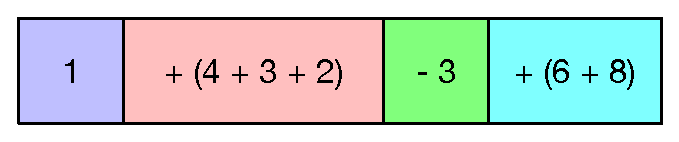
\includegraphics[width=0.35\linewidth]{images/basic_calculator_1}
	\caption{Basic Calculator I}
	\label{fig:basiccalculator1}
\end{figure}

\section{LC 0227 - Basic Calculator II}
Given a string {\colorbox{CodeBackground}{\lstinline|s|}} which represents an expression, evaluate this expression and return its value. \\

The integer division should truncate toward zero.\\

You may assume that the given expression is always valid. All intermediate results will be in the range of {\colorbox{CodeBackground}{\lstinline|[-2^31, 2^31 - 1]|}}.\\

Note: You are not allowed to use any built-in function which evaluates strings as mathematical expressions, such as {\colorbox{CodeBackground}{\lstinline|eval()|}}. \\

Constraints:
\begin{itemize}
	\item {\colorbox{CodeBackground}{\lstinline|1 <= s.length <= 3 * 10^5|}}
	\item {\colorbox{CodeBackground}{\lstinline|s|}} consists of integers and operators ({\colorbox{CodeBackground}{\lstinline|+|}}, {\colorbox{CodeBackground}{\lstinline|-|}}, {\colorbox{CodeBackground}{\lstinline|*|}}, {\colorbox{CodeBackground}{\lstinline|/|}}) separated by some number of spaces.
	\item {\colorbox{CodeBackground}{\lstinline|s|}} represents a valid expression.
	\item All the integers in the expression are non-negative integers in the range {\colorbox{CodeBackground}{\lstinline|[0, 2^31 - 1]|}}.
	\item The answer is guaranteed to fit in a 32-bit integer.
\end{itemize}

Examples:
\begin{itemize}
	\item {\colorbox{CodeBackground}{\lstinline|"3+2*2"\ \ --> 7|}}
	\item {\colorbox{CodeBackground}{\lstinline|" 3/2 "\ \ --> 1|}}
	\item {\colorbox{CodeBackground}{\lstinline|" 3+5 / 2 "\ \ --> 5|}}
\end{itemize}


\subsection*{Solution}
\begin{lstlisting}
#include <stack>
#include <string>

int calculate(std::string s) {
	std::stack<int> stk;
	long long currentNumber = 0;
	char operation = '+';
	for (int i = 0; i < s.length(); i++) {
		char currentChar = s[i];
		if (isdigit(currentChar)) { currentNumber = (currentNumber * 10) + (currentChar - '0'); }
		if (!isdigit(currentChar) && !isspace(currentChar) || i == s.length() - 1) {
			if (operation == '-') {
				stk.push(-currentNumber);
			} else if (operation == '+') {
				stk.push(currentNumber);
			} else if (operation == '*') {
				int stackTop = stk.top();
				stk.pop();
				stk.push(stackTop * currentNumber);
			} else if (operation == '/') {
				int stackTop = stk.top();
				stk.pop();
				stk.push(stackTop / currentNumber);
			}
			operation = currentChar;  // save the current operation
			currentNumber = 0;        // reset number for next iteration
		}
	}
	int result = 0;
	while (!stk.empty()) {
		result += stk.top();
		stk.pop();
	}
	return result;
}
\end{lstlisting}

\chapter{Monotonic Stack}

\section{LC 0739 - Daily Temperatures}
Given an array of integers {\colorbox{CodeBackground}{\lstinline|temperatures|}} represents the daily temperatures, return an array {\colorbox{CodeBackground}{\lstinline|answer|}} such that {\colorbox{CodeBackground}{\lstinline|answer[i]|}} is the number of days you have to wait after the {\colorbox{CodeBackground}{\lstinline|i|}}th day to get a warmer temperature. If there is no future day for which this is possible, keep {\colorbox{CodeBackground}{\lstinline|answer[i] == 0|}} instead.\\

Examples:
\begin{itemize}
\item {\colorbox{CodeBackground}{\lstinline|temperatures = [73,74,75,71,69,72,76,73] --> [1,1,4,2,1,1,0,0]|}}
\item {\colorbox{CodeBackground}{\lstinline|temperatures = [30,40,50,60] --> [1,1,1,0]|}}
\item {\colorbox{CodeBackground}{\lstinline|temperatures = [30,60,90] --> [1,1,0]|}}
\end{itemize}

\subsection*{Solution - Monotonic Stack}
\begin{lstlisting}
std::vector<int> dailyTemperatures(std::vector<int>& temperatures) {
  std::vector<int> num_days(temperatures.size(), 0);
  std::stack<int> stk;
  for (int i = 0; i < temperatures.size(); ++i) {
    while (!stk.empty() && temperatures[i] > temperatures[stk.top()]) {
      int top = stk.top();
      stk.pop();
      num_days[top] = i - top;
    }
    stk.push(i);
  }
  return num_days;
}
\end{lstlisting}

\section{LC 0496 - Next Greater Element I}
You are given two {\colorbox{CodeBackground}{\lstinline|0|}}-indexed integer arrays {\colorbox{CodeBackground}{\lstinline|nums1|}} and {\colorbox{CodeBackground}{\lstinline|nums2|}} \ul{without duplicates}, where {\colorbox{CodeBackground}{\lstinline|nums1|}} is a subset of {\colorbox{CodeBackground}{\lstinline|nums2|}}. \\

 For every integer in {\colorbox{CodeBackground}{\lstinline|nums1|}}, return the \ul{next greater number} in {\colorbox{CodeBackground}{\lstinline|nums2|}}. If there is no such \ul{next greater element} in {\colorbox{CodeBackground}{\lstinline|nums2|}}, return {\colorbox{CodeBackground}{\lstinline|-1.|}}.\\
 
 Explanation: For each {\colorbox{CodeBackground}{\lstinline|0 <= i < nums1.size()|}}, find the index {\colorbox{CodeBackground}{\lstinline|j|}} such that {\colorbox{CodeBackground}{\lstinline|nums1[i] == nums2[j]|}} and determine the \ul{next greater element} of {\colorbox{CodeBackground}{\lstinline|nums2[j]|}} in {\colorbox{CodeBackground}{\lstinline|nums2|}}. Return {\colorbox{CodeBackground}{\lstinline|-1|}} is there is no such \ul{next greater number} in {\colorbox{CodeBackground}{\lstinline|nums2|}}.\\

The \ul{next greater element} of some element {\colorbox{CodeBackground}{\lstinline|x|}} in an array is the first greater element that is to the right of {\colorbox{CodeBackground}{\lstinline|x|}} in the same array.\\

Examples:
\begin{itemize}
\item {\colorbox{CodeBackground}{\lstinline|nums1 = [4,1,2], nums2 = [1,3,4,2] --> [-1,3,-1]|}}\\
The next greater element for each value of {\colorbox{CodeBackground}{\lstinline|nums1|}} is as follows:\\
- {\colorbox{CodeBackground}{\lstinline|4|}} is underlined in $nums2 = [1,3,\underline{4},2]$ There is no next greater element, so the answer is {\colorbox{CodeBackground}{\lstinline|-1|}}.\\
- {\colorbox{CodeBackground}{\lstinline|1|}} is underlined in $nums2 = [\underline{1},3,4,2]$. The next greater element is {\colorbox{CodeBackground}{\lstinline|3|}}.\\
- {\colorbox{CodeBackground}{\lstinline|2|}} is underlined in $nums2 = [1,3,4,\underline{2}]$. There is no next greater element, so the answer is {\colorbox{CodeBackground}{\lstinline|-1|}}.
\item {\colorbox{CodeBackground}{\lstinline|nums1 = [2,4], nums2 = [1,2,3,4] --> [3,-1]|}}\\
The next greater element for each value of {\colorbox{CodeBackground}{\lstinline|nums1|}} is as follows:\\
- {\colorbox{CodeBackground}{\lstinline|2|}} is underlined in $nums2 = [1,\underline{2},3,4]$. The next greater element is {\colorbox{CodeBackground}{\lstinline|3|}}.\\
- {\colorbox{CodeBackground}{\lstinline|4|}} is underlined in $nums2 = [1,2,3,\underline{4}]$. There is no next greater element, so the answer is {\colorbox{CodeBackground}{\lstinline|-1|}}.
\end{itemize}

\subsection*{Solution - Monotonic Stack}
\begin{lstlisting}
std::vector<int> nextGreaterElement(std::vector<int>& nums1, std::vector<int>& nums2) {
  std::stack<int> stk;
  std::unordered_map<int, int> num2next_greater;
  for (int num : nums2) {
    while (!stk.empty() && num > stk.top()) {
      num2next_greater[stk.top()] = num;
      stk.pop();
    }
    stk.push(num);
  }
  std::vector<int> result;
  for (int num : nums1) {
    if (num2next_greater.find(num) != num2next_greater.end()) {
      result.push_back(num2next_greater[num]);
    } else {
      result.push_back(-1);
    }
  }
  return result;
}
\end{lstlisting}

\section{LC 0503 - Next Greater Element II}
Given a \ul{circular} integer array {\colorbox{CodeBackground}{\lstinline|nums|}} (i.e., the next element of {\colorbox{CodeBackground}{\lstinline|nums.back()|}} is {\colorbox{CodeBackground}{\lstinline|nums.front()|}}), return the \ul{next greater number} for every element in {\colorbox{CodeBackground}{\lstinline|nums|}}.\\

The \ul{next greater number} of a number {\colorbox{CodeBackground}{\lstinline|x|}} is the first greater number to its traversing-order next in the array, which means you could search circularly to find its next greater number. If it doesn't exist, return {\colorbox{CodeBackground}{\lstinline|-1|}} for this number.\\

Examples:
\begin{itemize}
\item {\colorbox{CodeBackground}{\lstinline|nums = [1,2,1] --> [2,-1,2]|}}\\
The first {\colorbox{CodeBackground}{\lstinline|1|}}'s next greater number is {\colorbox{CodeBackground}{\lstinline|2|}}. \\
The number {\colorbox{CodeBackground}{\lstinline|2|}} can't find next greater number. \\
The second {\colorbox{CodeBackground}{\lstinline|1|}}'s next greater number needs to search circularly, which is also {\colorbox{CodeBackground}{\lstinline|2|}}.
\item {\colorbox{CodeBackground}{\lstinline|nums = [1,2,3,4,3] --> [2,3,4,-1,4]|}}
\end{itemize}

\subsection*{Solution - Monotonic Stack}
\begin{lstlisting}
std::vector<int> nextGreaterElements(std::vector<int>& nums) {
  int n = nums.size();
  std::vector<int> result(n, -1);
  std::stack<int> stk;
  for (int i = 0; i < n * 2; ++i) {
    int num = nums[i % n];
    while (!stk.empty() && num > nums[stk.top()]) {
      result[stk.top()] = num;
      stk.pop();
    }
    if (i < n) { stk.push(i); }
  }
  return result;
}
\end{lstlisting}

\section{LC 0042 - Trapping Rain Water}
Given {\colorbox{CodeBackground}{\lstinline|n|}} ({\colorbox{CodeBackground}{\lstinline|n >= 1|}}) non-negative integers representing an elevation map where the width of each bar is {\colorbox{CodeBackground}{\lstinline|1|}}, compute how much water it can trap after raining.\\

Example: {\colorbox{CodeBackground}{\lstinline|height = [0,1,0,2,1,0,1,3,2,1,2,1] --> 6|}}
\begin{figure}[H]
\centering
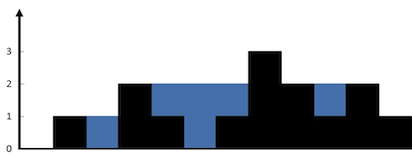
\includegraphics[width=0.4\linewidth]{images/lc0042_eg}
\end{figure}

\subsection*{Solution - Monotonic Stack}\label{solution:lc0042_monotonic_stack}
\begin{lstlisting}
int trap(std::vector<int>& heights) {
  std::stack<int> stk;
  int trapped_water = 0;
  int i = 0;
  while (i < heights.size()) {
    while (!stk.empty() && heights[i] > heights[stk.top()]) {
      int top = stk.top();
      stk.pop();
      if (stk.empty()) { break; }
      int width = i - stk.top() - 1;
      int height = std::min(heights[i], heights[stk.top()]) - heights[top];
      trapped_water += width * height;
    }
    stk.push(i);
    ++i;
  }
  return trapped_water;
}
\end{lstlisting}

\subsection*{Other Solutions}
\begin{itemize}
\item \hyperref[solution:lc0042_brute_force]{Brute Force (Time Limit Exceeded)}
\item \hyperref[solution:lc0042_brute_force_optimized_1]{Brute Force, Optimized 1}
\item \hyperref[solution:lc0042_brute_force_optimized_2]{Brute Force, Optimized 2}
%\item \hyperref[solution:lc0042_monotonic_stack]{Monotonic Stack}
\end{itemize}

\section{LC 0084 - Largest Rectangle in Histogram}
Given an array of integers {\colorbox{CodeBackground}{\lstinline|heights|}} representing the histogram's bar height where the width of each bar is {\colorbox{CodeBackground}{\lstinline|1|}}, return the area of the largest rectangle in the histogram.

\begin{itemize}
\item Example 1: {\colorbox{CodeBackground}{\lstinline|heights = [2,1,5,6,2,3] --> 10|}}
\begin{figure}[H]
\centering
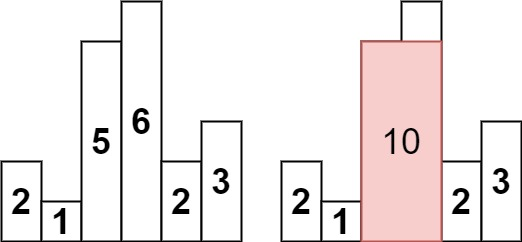
\includegraphics[width=0.3\linewidth]{images/lc0084_eg1}
\label{fig:lc0084eg1}
\end{figure}
\item Example 2: {\colorbox{CodeBackground}{\lstinline|heights = [2,4] --> 4|}}
\begin{figure}[H]
\centering
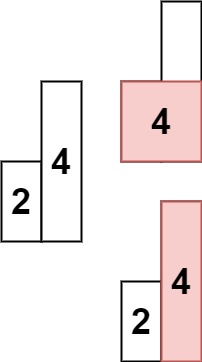
\includegraphics[width=0.11\linewidth]{images/lc0084_eg2}
\label{fig:lc0084eg2}
\end{figure}
\end{itemize}

\subsection*{Solution - Monotonic Stack}
\begin{lstlisting}
int largestRectangleArea(std::vector<int>& heights) {
  std::stack<int> s;
  int max_area = 0;
  for (int i = 0; i <= heights.size(); ++i) {
    int h = (i == heights.size() ? 0 : heights[i]);
    if (s.empty() || h >= heights[s.top()]) {
      s.push(i);
    } else {
      int tp = s.top();
      s.pop();
      int width = s.empty() ? i : i - s.top() - 1;
      max_area = std::max(max_area, heights[tp] * width);
      i--;
    }
  }
  return max_area;
}
\end{lstlisting}